\documentclass[conference]{IEEEtran}
\IEEEoverridecommandlockouts
% The preceding line is only needed to identify funding in the first footnote. If that is unneeded, please comment it out.
\usepackage{cite}
\usepackage{amsmath,amssymb,amsfonts}
\usepackage{algorithmic}
\usepackage{graphicx}
\usepackage{textcomp}
\usepackage{xcolor}
% --- Añadido para las secciones Diseño del Sistema / Composición del Prompt (diagramas, tablas, código) ---
\usepackage[utf8]{inputenc}
\usepackage[T1]{fontenc}
\usepackage{booktabs}
\usepackage{listings}
\usepackage{subcaption}
\usepackage{tikz}
\usetikzlibrary{arrows.meta,positioning,fit,backgrounds,shapes.geometric,calc}
\lstdefinestyle{promptbox}{
  basicstyle=\scriptsize\ttfamily,
  breaklines=true,
  breakatwhitespace=false,
  columns=fullflexible,
  keepspaces=true,
  frame=single,
  framerule=0.3pt,
  framesep=5pt,
  xleftmargin=6pt,
  xrightmargin=3pt,
  aboveskip=6pt,
  belowskip=4pt,
  extendedchars=true,
  literate=
    {á}{{\'a}}1 {é}{{\'e}}1 {í}{{\'i}}1 {ó}{{\'o}}1 {ú}{{\'u}}1
    {Á}{{\'A}}1 {É}{{\'E}}1 {Í}{{\'I}}1 {Ó}{{\'O}}1 {Ú}{{\'U}}1
    {ñ}{{\~n}}1 {Ñ}{{\~N}}1 {ü}{{\"u}}1 {¿}{{\textquestiondown}}1 {¡}{{\textexclamdown}}1,
}
\renewcommand{\tablename}{TABLA}
\renewcommand{\lstlistingname}{Listado}
% ------------------------------------------------------------------------------------
\def\BibTeX{{\rm B\kern-.05em{\sc i\kern-.025em b}\kern-.08em
    T\kern-.1667em\lower.7ex\hbox{E}\kern-.125emX}}
\begin{document}

\title{Hacia un Tutor Conversacional basado en LLM para la Programación con Scratch en Niños
}

\author{\IEEEauthorblockN{1\textsuperscript{er} Nombre Apellido}
\IEEEauthorblockA{\textit{dpto. nombre de la organización (de Afil.)} \\
\textit{nombre de la organización (de Afil.)}\\
Ciudad, País \\
correo electrónico u ORCID}
\and
\IEEEauthorblockN{2\textsuperscript{o} Nombre Apellido}
\IEEEauthorblockA{\textit{dpto. nombre de la organización (de Afil.)} \\
\textit{nombre de la organización (de Afil.)}\\
Ciudad, País \\
correo electrónico u ORCID}
\and
\IEEEauthorblockN{3\textsuperscript{er} Nombre Apellido}
\IEEEauthorblockA{\textit{dpto. nombre de la organización (de Afil.)} \\
\textit{nombre de la organización (de Afil.)}\\
Ciudad, País \\
correo electrónico u ORCID}
\and
\IEEEauthorblockN{4\textsuperscript{o} Nombre Apellido}
\IEEEauthorblockA{\textit{dpto. nombre de la organización (de Afil.)} \\
\textit{nombre de la organización (de Afil.)}\\
Ciudad, País \\
correo electrónico u ORCID}
\and
\IEEEauthorblockN{5\textsuperscript{o} Nombre Apellido}
\IEEEauthorblockA{\textit{dpto. nombre de la organización (de Afil.)} \\
\textit{nombre de la organización (de Afil.)}\\
Ciudad, País \\
correo electrónico u ORCID}
\and
\IEEEauthorblockN{6\textsuperscript{o} Nombre Apellido}
\IEEEauthorblockA{\textit{dpto. nombre de la organización (de Afil.)} \\
\textit{nombre de la organización (de Afil.)}\\
Ciudad, País \\
correo electrónico u ORCID}
}

\maketitle

\begin{abstract}
Este documento es un modelo e instrucciones para \LaTeX.
Este archivo, junto con el archivo IEEEtran.cls, define los componentes de su artículo [título, texto, encabezados, etc.]. *CRÍTICO: No use símbolos, caracteres especiales, notas al pie
ni fórmulas matemáticas en el título o el resumen del artículo.
\end{abstract}

\begin{IEEEkeywords}
componente, formato, estilo, estilizado, insertar
\end{IEEEkeywords}

\section{Introducción}
El pensamiento computacional (PC) se ha consolidado como una competencia fundamental para el siglo XXI, y abarca la descomposición de problemas, la abstracción, el reconocimiento de patrones y el razonamiento algorítmico [Wing, 2006]. Introducir el PC en la educación primaria se ha vuelto una prioridad global, y los entornos de programación visual como Scratch [Resnick et al., 2009] han demostrado ser eficaces para desarrollar estas habilidades en los estudiantes más jóvenes, pues ofrecen un punto de entrada de bajo umbral en el que los niños construyen programas conectando bloques en lugar de escribir texto. El marco de Brennan y Resnick [2012] identifica los conceptos, las prácticas y las perspectivas computacionales que surgen de este tipo de construcción, y se ha convertido en una perspectiva ampliamente adoptada para evaluar el desarrollo del PC en la niñez.
A pesar de la accesibilidad de Scratch, desarrollar el PC en el aula sigue siendo un desafío. Con frecuencia, un instructor acompaña a muchos niños a la vez, y las peticiones de ayuda se acumulan más rápido de lo que puede atenderlas una por una. Los estudiantes que se confunden o se atascan suelen perder el interés antes de recibir orientación, y los instructores señalan la dificultad de identificar qué niños necesitan atención inmediata. El andamiaje individualizado, reconocido como central para un aprendizaje eficaz [Wood et al., 1976; VanLehn, 2011], resulta difícil de sostener en estas condiciones, sobre todo con niños de 8 a 10 años, cuyas habilidades metacognitivas aún se están formando y que quizá no sepan pedir ayuda de forma productiva.
Los grandes modelos de lenguaje (LLM) abren la oportunidad de complementar la atención del instructor mediante una tutoría conversacional alineada con las metas de aprendizaje del PC. Trabajos recientes han explorado tutores basados en LLM para la enseñanza de la programación [CITE 1-2], pero la mayoría se dirige a estudiantes adultos, a lenguajes textuales, o supone una fluidez de tecleo y unas habilidades metacognitivas que los niños de primaria todavía no han desarrollado del todo. Diseñar un tutor con LLM que apoye el desarrollo del PC en este grupo de edad plantea desafíos propios: (i) la capacidad expresiva del niño está limitada por el tecleo y el vocabulario, lo que exige una interacción con andamiaje en lugar de un diálogo abierto; (ii) el tutor debe reconocer en qué etapa del proceso de construcción del PC se encuentra el niño y responder de forma adecuada sin desplazar su razonamiento; y (iii) el tutor debe operar dentro de restricciones de costo ajustadas para ser sostenible en programas educativos a gran escala.
La incorporación de LLM en contextos educativos también ha suscitado inquietudes. Se ha argumentado que depender de respuestas generadas por IA puede reducir las oportunidades de esfuerzo productivo Kirschner \& Hendrick, 2020, debilitar la implicación metacognitiva y fomentar la descarga cognitiva de maneras que erosionan la adquisición de habilidades a largo plazo [Gerlich, 2025; Kosmyna et al., 2025]. En la enseñanza de la programación en particular, distintos estudios han documentado que el acceso sin restricciones a asistentes que generan código puede llevar a los estudiantes a aceptar soluciones sin comprenderlas, lo que socava habilidades centrales del PC como la descomposición y la depuración [CITE Prather et al.; Denny et al.]. Estas preocupaciones cobran especial relevancia con los estudiantes más jóvenes, cuyas habilidades de PC apenas se están formando y cuya dependencia del apoyo cognitivo externo puede volverse un hábito. Por ello, un tutor basado en LLM diseñado para esta población debe decidir con cuidado cuándo y cómo interviene, y priorizar el andamiaje por encima de la entrega de la solución para preservar el espacio del propio razonamiento del estudiante.
En este artículo presentamos el diseño y la evaluación técnica de un tutor conversacional web pensado para apoyar el desarrollo del PC en niños de 9 a 12 años mientras construyen proyectos de Scratch. Guiado por la teoría del andamiaje [Wood et al., 1976] y por las estrategias didácticas de predecir-observar-explicar [White \& Gunstone, 1992], y atento a los riesgos ya señalados, nuestro diseño articula cuatro fases explícitas de interacción (predecir, pista, confirmar, responder) y un mecanismo de pistas progresivas que apoya al estudiante sin revelar la solución de forma prematura. El sistema se implementa con salidas estructuradas del LLM y sugerencias de bloques validadas para evitar la alucinación, y su huella de tokens se optimiza para un despliegue sostenible.


\section{Trabajos Relacionados}
\section{Diseño del Sistema}

El tutor se concibe como un sistema integrado que combina cuatro componentes: la interfaz de usuario (UI), la lógica de interacción, la representación del ejercicio y el prompt del LLM. Estos componentes se diseñaron en conjunto para mantener al tutor centrado en la tarea de programación actual del estudiante y ofrecer una orientación consistente.

Cuatro decisiones de diseño guiaron la implementación.
Interacción acotada al ejercicio. El tutor atiende un solo ejercicio de programación a la vez, en lugar de actuar como un asistente de programación de propósito general. Cada ejercicio define el objetivo de aprendizaje, los conceptos de pensamiento computacional relevantes y la estrategia de solución esperada. Acotar la interacción a este contexto mantiene al tutor centrado en la tarea actual del estudiante, reduce la conversación fuera de tema y facilita evaluar la retroalimentación generada frente a objetivos de aprendizaje bien definidos.

Salida estructurada y validada. El tutor nunca devuelve solo texto libre. Cada turno produce un objeto tipado que lleva una fase pedagógica, un mensaje breve para el niño, un conjunto opcional de bloques de Scratch para mostrar y dos o tres opciones de respuesta. El modelo recibe el catálogo completo de bloques disponibles y solo puede nombrar bloques que aparezcan en él; después, el backend elimina cualquier bloque que el modelo invente antes de que la respuesta llegue al niño. Así, cada sugerencia se mantiene fiel al entorno de Scratch y se evita que el tutor señale instrucciones que no existen.

Andamiaje por fases con pistas progresivas. La interacción se organiza en torno a cuatro fases que siguen la forma en que un tutor humano hace avanzar al estudiante: predecir, pista, confirmar y responder. Cuando un niño pide ayuda, el tutor primero lo invita a predecir qué hace un bloque; si el niño sigue atascado, libera pistas cada vez más concretas, desde un empujón hacia una categoría de bloques, pasando por una descripción del bloque que conviene usar, hasta mostrar el bloque como último paso. Una solución de referencia guía esta escalada, pero se mantiene oculta al niño, de modo que el estudiante conserva la autoría del razonamiento en lugar de recibir la respuesta.

Operación consciente de la latencia y el costo. Los estudiantes más jóvenes pierden el interés cuando una respuesta tarda demasiado, así que el sistema prefiere un modelo rápido con un prompt compacto antes que uno más grande y lento. Cada solicitud lleva solo los últimos 14 mensajes de la conversación, un catálogo de bloques recortado y una temperatura de muestreo baja. Desplegamos Gemini~2.5~Flash en lugar de un modelo más orientado al razonamiento porque el tiempo adicional de deliberación de este último llevaba la latencia de respuesta más allá de lo que un niño de esta edad está dispuesto a esperar, sin una mejora equivalente en la calidad de la tutoría para estos intercambios breves. El backend, además, registra el número de tokens de entrada y de salida por mensaje, lo que hace medible el costo de operación y mantiene el diseño responsable frente a la restricción de sostenibilidad planteada en la introducción.

\subsection{Arquitectura}

La Fig.~\ref{fig:arch} muestra la arquitectura en ejecución. El frontend es una aplicación de página única (SPA) en React construida con Vite. En lugar de una estructura basada en rutas, ejecuta una pequeña máquina de estados de cinco pantallas (bienvenida, asentimiento, selección de juego, chat y retroalimentación) que mantiene en memoria la conversación y la sesión activas, y llega al backend a través de un único cliente de API tipado. Esto mantiene el recorrido del niño por la aplicación lineal y predecible, algo que importa para un público de entre ocho y diez años.

El backend es un servicio en FastAPI organizado en cuatro capas, cada una con una sola responsabilidad: las rutas exponen la superficie HTTP bajo \texttt{/api/v1}, los servicios contienen la lógica de tutoría, los repositorios concentran todo el acceso a la base de datos y los modelos definen el esquema mediante un mapeo asíncrono de SQLAlchemy. La lógica de tutoría depende de una interfaz \texttt{TutorLLM} agnóstica al proveedor, y una fábrica selecciona el proveedor concreto en tiempo de ejecución a partir de un único indicador de configuración. Las sesiones, las conversaciones, los mensajes y la retroalimentación anónima persisten en PostgreSQL en producción y en SQLite durante el desarrollo, sin ningún cambio en el código de la aplicación. En una instalación desplegada, nginx sirve el frontend compilado y hace de proxy de \texttt{/api/} hacia el backend, de modo que el navegador se comunica con un solo origen.

La Fig.~\ref{fig:sequence} traza un turno. El niño toca una opción de respuesta o escribe un mensaje; el frontend lo envía al endpoint de la conversación; el servicio persiste el mensaje del niño, arma el prompt descrito en la Sección~\ref{sec:prompt} y llama al modelo elegido; la respuesta se valida frente al catálogo de bloques, se guarda junto con su fase y su conteo de tokens, y se devuelve al frontend, que muestra el mensaje junto con su insignia de fase, las tarjetas de bloque que correspondan y el siguiente conjunto de opciones de respuesta.

\begin{figure*}[!t]
\centering
\resizebox{\textwidth}{!}{%
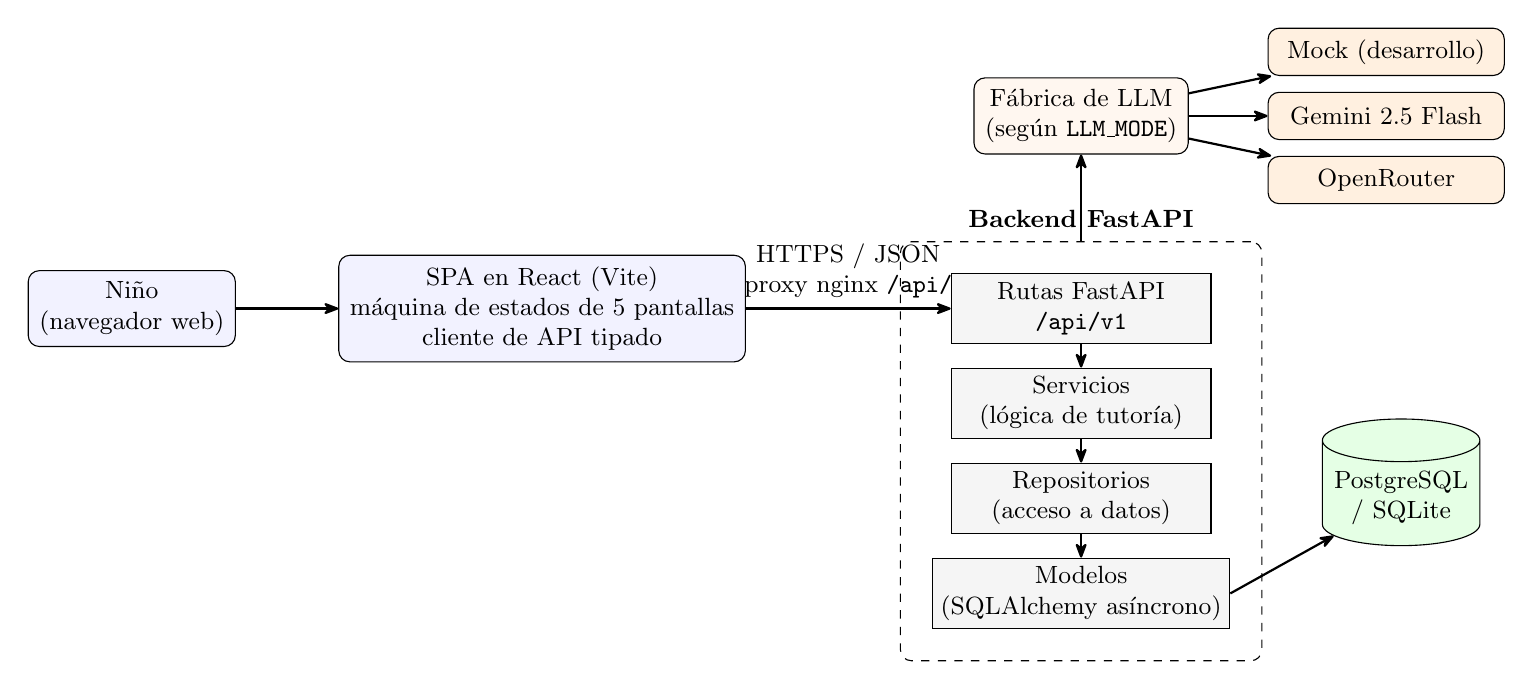
\begin{tikzpicture}[
  font=\small,
  >={Stealth[round]},
  box/.style={draw, rounded corners, align=center, minimum height=9mm, inner sep=4pt, fill=blue!5},
  layer/.style={draw, align=center, minimum width=33mm, minimum height=7mm, fill=gray!8, inner sep=3pt},
  db/.style={draw, cylinder, shape border rotate=90, aspect=0.28, align=center, minimum height=13mm, minimum width=20mm, fill=green!10},
  prov/.style={draw, rounded corners, align=center, minimum width=30mm, minimum height=6mm, fill=orange!12, inner sep=2pt},
  arr/.style={-{Stealth[round]}, thick},
]
% cliente
\node[box] (child) {Niño\\(navegador web)};
\node[box, right=13mm of child] (spa) {SPA en React (Vite)\\máquina de estados de 5 pantallas\\cliente de API tipado};
% capas internas del backend
\node[layer, right=26mm of spa] (routes) {Rutas FastAPI\\\texttt{/api/v1}};
\node[layer, below=3mm of routes] (svc) {Servicios\\(lógica de tutoría)};
\node[layer, below=3mm of svc] (repo) {Repositorios\\(acceso a datos)};
\node[layer, below=3mm of repo] (model) {Modelos\\(SQLAlchemy asíncrono)};
\begin{scope}[on background layer]
\node[draw, dashed, rounded corners, fit=(routes)(svc)(repo)(model), inner sep=4mm] (be) {};
\end{scope}
\node[above=0.5mm of be.north] {\textbf{Backend FastAPI}};
% persistencia
\node[db, right=14mm of repo] (dbn) {PostgreSQL\\/ SQLite};
% proveedores LLM
\node[box, above=11mm of be.north, fill=orange!6] (factory) {Fábrica de LLM\\(según \texttt{LLM\_MODE})};
\node[prov, right=10mm of factory] (gem) {Gemini 2.5 Flash};
\node[prov, above=2mm of gem] (mock) {Mock (desarrollo)};
\node[prov, below=2mm of gem] (orr) {OpenRouter};
% flechas
\draw[arr] (child) -- (spa);
\draw[arr] (spa) -- node[above, align=center]{HTTPS / JSON\\proxy nginx \texttt{/api/}} (routes.west);
\draw[arr] (routes) -- (svc);
\draw[arr] (svc) -- (repo);
\draw[arr] (repo) -- (model);
\draw[arr] (model.east) -- (dbn);
\draw[arr] (be.north) -- (factory.south);
\draw[arr] (factory) -- (gem);
\draw[arr] (factory) -- (mock);
\draw[arr] (factory) -- (orr);
\end{tikzpicture}%
}
\caption{Arquitectura en ejecución. Una aplicación de página única en React guía un flujo lineal de cinco pantallas y se comunica con un backend en FastAPI por capas mediante JSON. La lógica de tutoría llama a una interfaz de modelo de lenguaje agnóstica al proveedor, cuya implementación concreta se selecciona con un único indicador de configuración; las sesiones y los mensajes persisten en PostgreSQL en producción y en SQLite en desarrollo.}
\label{fig:arch}
\end{figure*}

\begin{figure}[!t]
\centering
\resizebox{\columnwidth}{!}{%
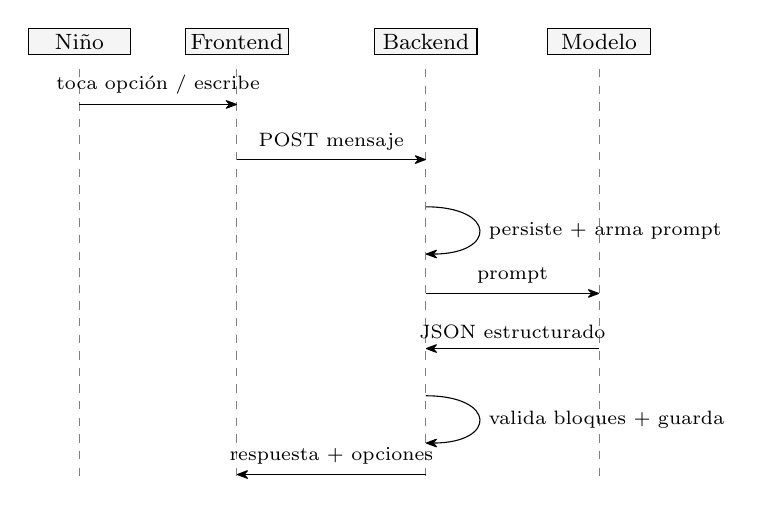
\begin{tikzpicture}[font=\footnotesize, >={Stealth[round]}]
% líneas de vida
\foreach \x/\lbl in {0/Niño, 2.0/Frontend, 4.4/Backend, 6.6/Modelo}{
  \node[draw, fill=gray!8, minimum width=13mm, inner sep=2pt] at (\x,0) {\lbl};
  \draw[dashed, gray] (\x,-0.35) -- (\x,-5.6);
}
\draw[-{Stealth[round]}] (0,-0.8) -- node[above, font=\scriptsize]{toca opción / escribe} (2.0,-0.8);
\draw[-{Stealth[round]}] (2.0,-1.5) -- node[above, font=\scriptsize]{POST mensaje} (4.4,-1.5);
% acción interna del backend
\draw[-{Stealth[round]}] (4.4,-2.1) .. controls (5.3,-2.1) and (5.3,-2.7) .. (4.4,-2.7)
  node[right, font=\scriptsize, pos=0.5]{persiste + arma prompt};
\draw[-{Stealth[round]}] (4.4,-3.2) -- node[above, font=\scriptsize]{prompt} (6.6,-3.2);
\draw[{Stealth[round]}-] (4.4,-3.9) -- node[above, font=\scriptsize]{JSON estructurado} (6.6,-3.9);
\draw[-{Stealth[round]}] (4.4,-4.5) .. controls (5.3,-4.5) and (5.3,-5.1) .. (4.4,-5.1)
  node[right, font=\scriptsize, pos=0.5]{valida bloques + guarda};
\draw[{Stealth[round]}-] (2.0,-5.5) -- node[above, font=\scriptsize]{respuesta + opciones} (4.4,-5.5);
\end{tikzpicture}%
}
\caption{Intercambio de mensajes en un turno. El backend persiste el mensaje del niño, arma el prompt por capas, llama al modelo y valida las sugerencias de bloques frente al catálogo antes de guardar y devolver la respuesta tipada.}
\label{fig:sequence}
\end{figure}

\subsection{Modelos de Lenguaje}
\label{sec:models}

El proveedor por defecto es Google Gemini~2.5~Flash. Se invoca con un esquema de salida estructurada nativo, de modo que el modelo queda obligado a emitir directamente el objeto de respuesta tipado en lugar de texto libre que el backend tendría que analizar. La temperatura de muestreo se mantiene en 0.3 para que el comportamiento de tutoría sea estable entre turnos. Un segundo proveedor enruta el mismo prompt a través de la API de OpenRouter con una interfaz compatible con OpenAI; como esa vía no expone un esquema nativo, el prompt añade una descripción explícita del objeto JSON requerido. Un proveedor simulado (mock) devuelve respuestas deterministas sin llamada de red y se usa en el desarrollo local y en las pruebas automatizadas. Los tres implementan la misma interfaz \texttt{TutorLLM} y son intercambiables por configuración, lo que nos permitió comparar proveedores sin tocar la lógica de tutoría.

\section{Composición del Prompt}
\label{sec:prompt}

El comportamiento del tutor depende casi por completo de cómo se arma el prompt. Cada solicitud combina una instrucción pedagógica fija, una descripción del ejercicio actual, el catálogo de bloques utilizables y la conversación reciente, y obliga al modelo a responder con un objeto tipado. La Tabla~\ref{tab:prompt} enumera estas partes, y la Fig.~\ref{fig:prompt} muestra cómo se disponen en capas dentro de una sola solicitud y cómo la respuesta regresa a la interfaz.

\begin{table}[!t]
\caption{Componentes del prompt ensamblado}
\label{tab:prompt}
\centering
\renewcommand{\arraystretch}{1.25}
\begin{tabular}{@{}p{1.9cm}p{1.4cm}p{3.5cm}@{}}
\toprule
\textbf{Componente} & \textbf{Alcance} & \textbf{Propósito} \\
\midrule
Base estática & Cada turno & Persona, política de cuatro fases, regla de pistas progresivas, reglas de bloques y de opciones de respuesta \\
Contexto del ejercicio & Por ejercicio & Título, instrucción al niño, objetivos, pistas; y, de forma privada, la solución de referencia y los ids de bloques clave \\
Catálogo de bloques & Cada turno & Los 47 bloques disponibles (id, nombre, descripción) como único vocabulario permitido \\
Transcripción & Cada turno & Los últimos 14 mensajes más el nuevo mensaje del niño \\
Esquema de salida & Cada turno & Seis campos tipados que el modelo debe devolver \\
\bottomrule
\end{tabular}
\end{table}

\begin{figure*}[!t]
\centering
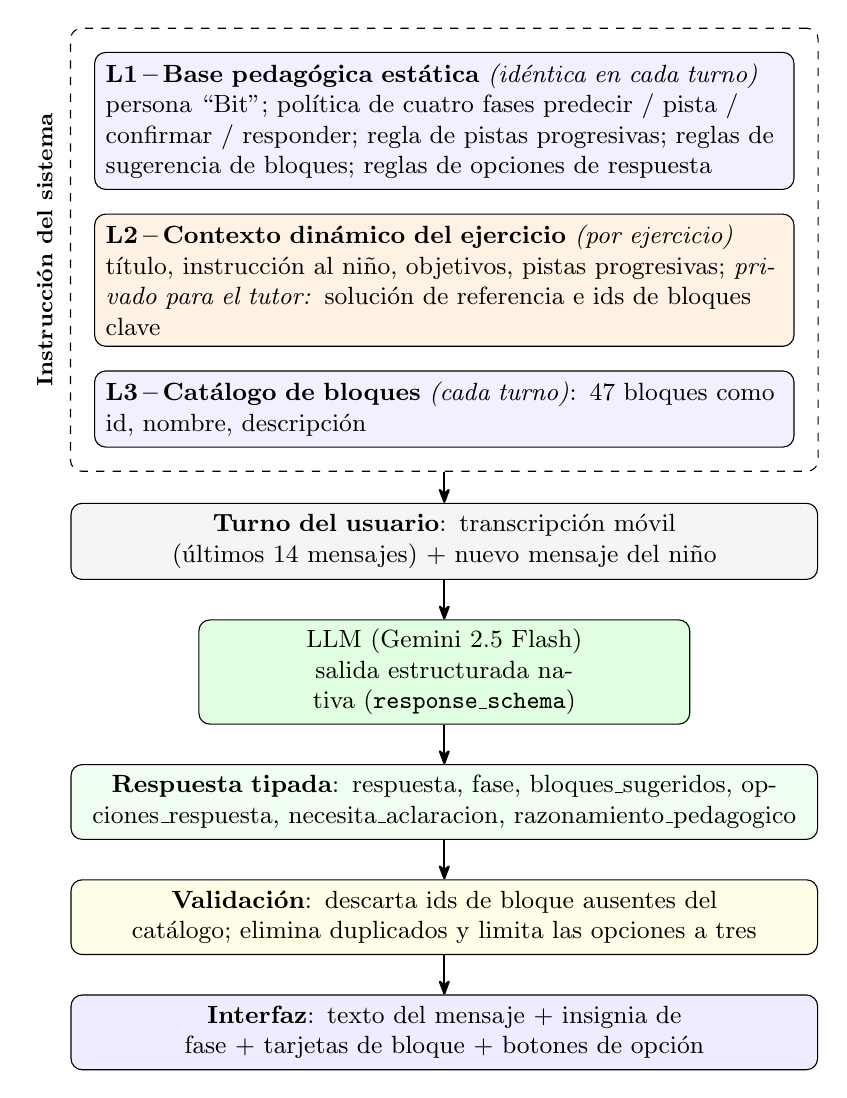
\begin{tikzpicture}[
  font=\small,
  >={Stealth[round]},
  node distance=3mm,
  layerA/.style={draw, rounded corners, align=left, text width=86mm, fill=blue!6, inner sep=4pt},
  layerB/.style={draw, rounded corners, align=left, text width=86mm, fill=orange!10, inner sep=4pt},
  io/.style={draw, rounded corners, align=center, text width=92mm, fill=gray!8, inner sep=4pt},
  llm/.style={draw, rounded corners, align=center, text width=60mm, fill=green!12, minimum height=9mm},
  arr/.style={-{Stealth[round]}, thick},
]
\node[layerA] (base) {\textbf{L1\,--\,Base pedagógica estática} \emph{(idéntica en cada turno)}\\ persona ``Bit''; política de cuatro fases predecir / pista / confirmar / responder; regla de pistas progresivas; reglas de sugerencia de bloques; reglas de opciones de respuesta};
\node[layerB, below=of base] (ctx) {\textbf{L2\,--\,Contexto dinámico del ejercicio} \emph{(por ejercicio)}\\ título, instrucción al niño, objetivos, pistas progresivas; \emph{privado para el tutor:} solución de referencia e ids de bloques clave};
\node[layerA, below=of ctx] (cat) {\textbf{L3\,--\,Catálogo de bloques} \emph{(cada turno)}: 47 bloques como id, nombre, descripción};
\begin{scope}[on background layer]
\node[draw, dashed, rounded corners, fit=(base)(ctx)(cat), inner sep=3mm] (sys) {};
\end{scope}
\node[left=1mm of sys.west, rotate=90, anchor=south, font=\footnotesize\bfseries] {Instrucción del sistema};
\node[io, below=7mm of cat] (turn) {\textbf{Turno del usuario}: transcripción móvil (últimos 14 mensajes) $+$ nuevo mensaje del niño};
\node[llm, below=5mm of turn] (llm) {LLM (Gemini 2.5 Flash)\\ salida estructurada nativa (\texttt{response\_schema})};
\node[io, below=5mm of llm, fill=green!6] (json) {\textbf{Respuesta tipada}: respuesta, fase, bloques\_sugeridos, opciones\_respuesta, necesita\_aclaracion, razonamiento\_pedagogico};
\node[io, below=5mm of json, fill=yellow!10] (val) {\textbf{Validación}: descarta ids de bloque ausentes del catálogo; elimina duplicados y limita las opciones a tres};
\node[io, below=5mm of val, fill=blue!7] (ui) {\textbf{Interfaz}: texto del mensaje $+$ insignia de fase $+$ tarjetas de bloque $+$ botones de opción};
\draw[arr] (sys.south) -- (turn.north);
\draw[arr] (turn) -- (llm);
\draw[arr] (llm) -- (json);
\draw[arr] (json) -- (val);
\draw[arr] (val) -- (ui);
\end{tikzpicture}
\caption{Composición del prompt y flujo de la respuesta. La instrucción del sistema se ensambla a partir de una base pedagógica estática, el contexto del ejercicio actual (cuya solución de referencia y bloques clave permanecen ocultos al niño) y el catálogo de bloques. Junto con la transcripción reciente conforma una sola solicitud; el modelo devuelve un objeto tipado que el backend valida frente al catálogo antes de que la interfaz lo muestre.}
\label{fig:prompt}
\end{figure*}

\subsection{Base Pedagógica Estática}

La base estática es la misma en cada turno y codifica la persona del tutor y sus reglas de interacción. Presenta al modelo como ``Bit'', un tutor de Scratch amable para niños, y enuncia con claridad la meta que lo gobierna: ayudar a que el estudiante comprenda, no resolver el ejercicio por él. Luego asigna situaciones habituales a las cuatro fases: por ejemplo, un saludo o una pregunta factual llevan a \emph{responder}, una primera petición de ayuda lleva a \emph{predecir}, y la dificultad repetida lleva a una \emph{pista} que escala. La base también fija restricciones de forma que importan para este público: frases cortas, a lo sumo un emoji, no mostrar más de un bloque por turno y un recordatorio explícito de que el tutor no puede ver la pantalla del niño y debe preguntar cuando necesita saber qué ha construido.

\subsection{Contexto Dinámico del Ejercicio}

Para cada ejercicio, el backend añade un bloque de contexto compacto. Siempre incluye el título, la instrucción dirigida al niño, los objetivos de aprendizaje y las pistas progresivas escritas por el autor. Cuando el ejercicio las define, agrega además dos campos marcados como privados que nunca deben revelarse por completo: una solución de referencia en lenguaje natural y una lista ordenada de ids de bloques clave. La solución de referencia funciona como una brújula para decidir el siguiente paso y la siguiente pregunta, y los bloques clave le indican al tutor qué ids priorizar cuando conviene sugerir. El Listado~\ref{lst:ctx} muestra este contexto para un ejercicio representativo, en el español que se usa en el despliegue.

\begin{lstlisting}[style=promptbox, caption={Contexto del ejercicio para un juego representativo (los ids de bloque son textuales).}, label={lst:ctx}]
EJERCICIO ACTUAL:
Título: Haz bailar al gato
Instrucción al niño: ¡Vamos a hacer bailar al gato!
  Primero piensa: ¿qué bloque hace que el programa
  empiece?
Objetivos: usar el evento bandera verde; mover y
  girar el personaje; usar repetición para animar.
Pistas progresivas:
  1) Fíjate en la categoría Eventos para arrancar.
  2) En Movimiento hay bloques que giran y mueven.
  3) Para que baile de verdad, usa Repetir de Control.

SOLUCIÓN DE REFERENCIA (solo para ti, no la reveles
  completa; úsala como brújula): al presionar la
  bandera verde, el gato se mueve a la derecha y luego
  a la izquierda varias veces con un bucle y pequeñas
  esperas; después gira sobre sí mismo y vuelve a
  mirar a la derecha.

BLOQUES CLAVE (solo para ti, prioriza estos ids,
  muestra uno por turno):
  - eventos_bandera_verde ("bandera verde")
  - movimiento_mover_pasos ("mover pasos")
  - movimiento_girar_derecha_grados ("girar a la derecha")
  - control_repetir_veces ("repetir veces")
  - control_por_siempre ("por siempre")
\end{lstlisting}

\subsection{Catálogo de Bloques y Anclaje contra Alucinaciones}

Cada solicitud lleva un catálogo recortado de los 47 bloques de Scratch que el tutor puede referenciar, cada uno con un id, un nombre visible y una descripción de una línea. El catálogo cumple dos propósitos. Le da al modelo un vocabulario cerrado para que las sugerencias se mantengan dentro de los bloques que el niño realmente tiene, y ancla los ids que el backend verifica después. Cuando el modelo responde, el backend conserva únicamente los bloques sugeridos cuyos ids aparecen en el catálogo y descarta el resto, de modo que un bloque inventado o mal escrito nunca llega a la interfaz. El mismo id sirve para localizar la imagen del bloque que ve el niño, lo que vincula la sugerencia textual con un elemento visual concreto de Scratch.

\subsection{Contrato de Salida Estructurada}

El prompt exige que el modelo responda con un único objeto tipado en lugar de prosa. Sus campos son el mensaje que se muestra al niño (\texttt{respuesta}), la fase pedagógica (\texttt{fase}), los bloques por mostrar (\texttt{bloques\_sugeridos}), las opciones de respuesta (\texttt{opciones\_respuesta}), un indicador de que el tutor necesita ver más antes de poder ayudar (\texttt{necesita\_aclaracion}) y una nota interna breve que explica la decisión pedagógica (\texttt{razonamiento\_pedagogico}), que se registra pero no se muestra. El Listado~\ref{lst:json} presenta el esquema. Como la fase forma parte de la salida, el tutor declara en cada turno en qué punto del ciclo de andamiaje se encuentra, algo que la interfaz muestra como una insignia de color y que, además, hace que cada turno sea analizable a posteriori. La Fig.~\ref{fig:phases} muestra las transiciones entre fases.

\begin{lstlisting}[style=promptbox, caption={Respuesta tipada que el modelo debe devolver.}, label={lst:json}]
{
  "respuesta": "texto que se muestra al niño",
  "fase": "predecir" | "pista" | "confirmar" | "responder",
  "bloques_sugeridos": [{"id": "...", "imagen": "...", "nombre": "..."}],
  "opciones_respuesta": ["...", "..."],
  "necesita_aclaracion": true | false,
  "razonamiento_pedagogico": "nota interna breve (no se muestra)"
}
\end{lstlisting}

\begin{figure}[!t]
\centering
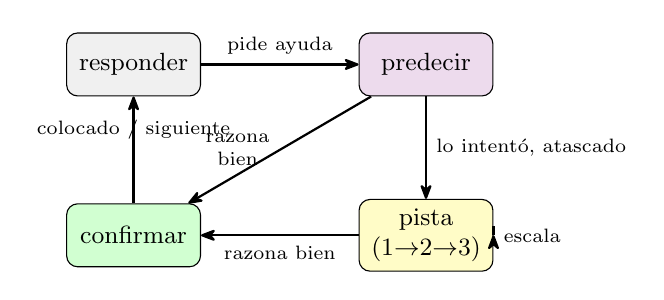
\begin{tikzpicture}[
  font=\small,
  >={Stealth[round]},
  st/.style={draw, rounded corners, align=center, minimum width=17mm, minimum height=8mm},
  arr/.style={-{Stealth[round]}, thick},
]
\node[st, fill=gray!12] (respond) {responder};
\node[st, fill=violet!14, right=20mm of respond] (predict) {predecir};
\node[st, fill=yellow!22, below=13mm of predict] (hint) {pista\\(1$\to$2$\to$3)};
\node[st, fill=green!18, left=20mm of hint] (confirm) {confirmar};
\draw[arr] (respond) -- node[above, font=\scriptsize]{pide ayuda} (predict);
\draw[arr] (predict) -- node[right, font=\scriptsize]{lo intentó, atascado} (hint);
\draw[arr] (hint.east) to[out=-35,in=35,looseness=6] node[right, font=\scriptsize]{escala} (hint.east);
\draw[arr] (hint) -- node[below, font=\scriptsize]{razona bien} (confirm);
\draw[arr] (predict) -- node[left, font=\scriptsize, align=center]{razona\\bien} (confirm);
\draw[arr] (confirm) -- node[above, font=\scriptsize]{colocado / siguiente} (respond);
\end{tikzpicture}
\caption{Fases de interacción. Una petición de ayuda lleva al tutor de \emph{responder} a \emph{predecir}; la dificultad sostenida escala las pistas de vagas a concretas; una vez que el niño razona correctamente, el tutor \emph{confirma} y muestra el bloque, y luego vuelve a \emph{responder}. Los turnos casuales o factuales permanecen en \emph{responder}.}
\label{fig:phases}
\end{figure}

\subsection{Representación por Proveedor}

La base pedagógica, el contexto del ejercicio, el catálogo de bloques y la transcripción se comparten entre proveedores, lo que mantiene consistente el comportamiento del tutor cuando cambia el modelo. Los dos proveedores solo difieren en cómo se impone el contrato de salida. A Gemini se le da el esquema como un formato de respuesta nativo, así que la restricción la aplica el entorno de ejecución del modelo. A OpenRouter, al que se accede por una interfaz compatible con OpenAI, se le entrega el mismo esquema como una instrucción explícita añadida a la base y se le pide que devuelva solo ese objeto. En ambos casos, el backend analiza el resultado, aplica la validación de bloques y de opciones descrita antes, y registra el proveedor, el modelo, la versión del prompt y el conteo de tokens junto al mensaje guardado.

\section{Características de Interacción}
\label{sec:features}

Cuatro características llevan el diseño de andamiaje a la interfaz. La Fig.~\ref{fig:ui} las ilustra en el sistema en funcionamiento.

\emph{Pistas progresivas.} Cuando un niño sigue atascado, el tutor no se repite ni revela la respuesta. Escala en tres niveles: desde un empujón hacia una categoría de bloques, a una descripción del bloque que hay que buscar, hasta mostrar el bloque; solo el último nivel coloca un bloque en la respuesta. La solución de referencia dirige la escalada mientras permanece oculta, de modo que el apoyo aumenta sin quitarle el trabajo al niño.

\emph{Opciones de respuesta como andamiaje.} Bajo cada mensaje del tutor, la interfaz muestra dos o tres botones cortos redactados con la voz del propio niño, por ejemplo ``El gato se mueve'' o ``Dame otra pista''. Los botones reducen el costo de responder para un estudiante que aún no teclea con fluidez, y una de las opciones siempre es una salida para el niño que no sabe, como ``No estoy seguro''. Se mantiene disponible un campo de texto libre para los niños que prefieren escribir su propia respuesta, de modo que las opciones guían sin encasillar.

\emph{Predecir y verificar.} Antes de dar por bueno un bloque, el tutor invita al niño a predecir qué hará y luego a probarlo ejecutando el programa. Así, cada bloque sugerido se convierte en un pequeño experimento en lugar de una instrucción que copiar, lo que mantiene al niño observando y razonando sobre el comportamiento en Scratch.

\emph{Sugerencias de bloques validadas.} Un bloque sugerido aparece como una tarjeta visual con la imagen del bloque y su nombre, tomada del mismo catálogo al que se restringe el modelo. Como el backend ya descartó cualquier id fuera del catálogo, el niño solo ve bloques que existen en su entorno, y la insignia de fase sobre el mensaje indica si el tutor está pidiendo una predicción, dando una pista o confirmando un paso.

El flujo que rodea a la interacción apoya el uso en el aula. Una sesión se reanuda de forma automática si el niño cierra el navegador antes de terminar, así que una interrupción no hace perder el progreso; una sesión se marca como completada solo cuando un instructor ingresa un código de administrador, lo que mantiene la finalización bajo su control; y cada ejercicio ofrece un video corto opcional que muestra un anticipo del proyecto terminado.

\begin{figure*}[!t]
\centering
% --- Capturas de la interacción: reemplaza los marcadores de abajo con capturas de la app en ejecución. ---
% Archivos esperados (colócalos junto a este .tex, p. ej. en ./fig/):
%   fig/ui_predict.png      fig/ui_hint_block.png      fig/ui_options.png      fig/ui_confirm.png
\begin{subfigure}[t]{0.48\textwidth}
  \centering
  \fbox{\rule{0pt}{42mm}\rule{0.9\linewidth}{0pt}} % marcador; bórralo al agregar la imagen
  % \includegraphics[width=0.95\linewidth]{fig/ui_predict.png}
  \caption{Fase predecir: el tutor muestra un bloque y pide al niño predecir qué hace; las opciones de respuesta aparecen debajo.}
  \label{fig:ui-predict}
\end{subfigure}
\hfill
\begin{subfigure}[t]{0.48\textwidth}
  \centering
  \fbox{\rule{0pt}{42mm}\rule{0.9\linewidth}{0pt}} % marcador; bórralo al agregar la imagen
  % \includegraphics[width=0.95\linewidth]{fig/ui_hint_block.png}
  \caption{Fase pista (nivel 3): tras una dificultad sostenida, el tutor muestra el bloque concreto como una tarjeta validada.}
  \label{fig:ui-hint}
\end{subfigure}

\vspace{3mm}

\begin{subfigure}[t]{0.48\textwidth}
  \centering
  \fbox{\rule{0pt}{42mm}\rule{0.9\linewidth}{0pt}} % marcador; bórralo al agregar la imagen
  % \includegraphics[width=0.95\linewidth]{fig/ui_options.png}
  \caption{Opciones de respuesta como andamiaje: botones con la voz del niño, incluida una opción de escape, con un campo de texto libre siempre disponible.}
  \label{fig:ui-options}
\end{subfigure}
\hfill
\begin{subfigure}[t]{0.48\textwidth}
  \centering
  \fbox{\rule{0pt}{42mm}\rule{0.9\linewidth}{0pt}} % marcador; bórralo al agregar la imagen
  % \includegraphics[width=0.95\linewidth]{fig/ui_confirm.png}
  \caption{Fase confirmar: una vez que el niño razona correctamente, el tutor confirma y muestra el bloque que corresponde.}
  \label{fig:ui-confirm}
\end{subfigure}
\caption{La interfaz del tutor durante una sesión (véase la Sección~\ref{sec:features}). Cada panel muestra una insignia de fase, el mensaje del tutor, las tarjetas de bloque validadas que correspondan y las opciones de respuesta que el niño puede tocar.}
\label{fig:ui}
\end{figure*}


\end{document}
